\documentclass[]{jarticle}          % 一段組
%\documentclass[twocolumn]{jarticle} % 二段組

\textwidth 180mm
\textheight 255mm
\oddsidemargin -12mm
\topmargin -15mm
\columnsep 10mm

%\vspace{0.5cm} % 一段組の場合はコメントアウトした方が体裁がよいx
%] % 一段組の場合はコメントアウトする

\usepackage{styles/labheadings}
\usepackage[dvipdfmx]{graphicx,color}
\usepackage{amsmath,amssymb}
\usepackage{url}
% 追加
\usepackage{listings,jvlisting}
\usepackage[hang,small,bf]{caption}
\usepackage[subrefformat=parens]{subcaption}
\captionsetup{compatibility=false}

\newcommand{\aU}{\mbox{\boldmath $a$}}
\newcommand{\bU}{\mbox{\boldmath $b$}}
\newcommand{\cU}{\mbox{\boldmath $c$}}
\newcommand{\dU}{\mbox{\boldmath $d$}}
\newcommand{\eU}{\mbox{\boldmath $e$}}
\newcommand{\fU}{\mbox{\boldmath $f$}}
\newcommand{\gU}{\mbox{\boldmath $g$}}
\newcommand{\hU}{\mbox{\boldmath $h$}}
\newcommand{\iU}{\mbox{\boldmath $i$}}
\newcommand{\jU}{\mbox{\boldmath $j$}}
\newcommand{\kU}{\mbox{\boldmath $k$}}
\newcommand{\lU}{\mbox{\boldmath $l$}}
\newcommand{\mU}{\mbox{\boldmath $m$}}
\newcommand{\nU}{\mbox{\boldmath $n$}}
\newcommand{\oU}{\mbox{\boldmath $o$}}
\newcommand{\pU}{\mbox{\boldmath $p$}}
\newcommand{\qU}{\mbox{\boldmath $q$}}
\newcommand{\rU}{\mbox{\boldmath $r$}}
\newcommand{\sU}{\mbox{\boldmath $s$}}
\newcommand{\tU}{\mbox{\boldmath $t$}}
\newcommand{\uU}{\mbox{\boldmath $u$}}
\newcommand{\vU}{\mbox{\boldmath $v$}}
\newcommand{\wU}{\mbox{\boldmath $w$}}
\newcommand{\xU}{\mbox{\boldmath $x$}}
\newcommand{\yU}{\mbox{\boldmath $y$}}
\newcommand{\zU}{\mbox{\boldmath $z$}}
\newcommand{\AU}{\mbox{\boldmath $A$}}
\newcommand{\BU}{\mbox{\boldmath $B$}}
\newcommand{\CU}{\mbox{\boldmath $C$}}
\newcommand{\DU}{\mbox{\boldmath $D$}}
\newcommand{\EU}{\mbox{\boldmath $E$}}
\newcommand{\FU}{\mbox{\boldmath $F$}}
\newcommand{\GU}{\mbox{\boldmath $G$}}
\newcommand{\HU}{\mbox{\boldmath $H$}}
\newcommand{\IU}{\mbox{\boldmath $I$}}
\newcommand{\JU}{\mbox{\boldmath $J$}}
\newcommand{\KU}{\mbox{\boldmath $K$}}
\newcommand{\LU}{\mbox{\boldmath $L$}}
\newcommand{\MU}{\mbox{\boldmath $M$}}
\newcommand{\NU}{\mbox{\boldmath $N$}}
\newcommand{\OU}{\mbox{\boldmath $O$}}
\newcommand{\PU}{\mbox{\boldmath $P$}}
\newcommand{\QU}{\mbox{\boldmath $Q$}}
\newcommand{\RU}{\mbox{\boldmath $R$}}
\newcommand{\SU}{\mbox{\boldmath $S$}}
\newcommand{\TU}{\mbox{\boldmath $T$}}
\newcommand{\UU}{\mbox{\boldmath $U$}}
\newcommand{\VU}{\mbox{\boldmath $V$}}
\newcommand{\WU}{\mbox{\boldmath $W$}}
\newcommand{\XU}{\mbox{\boldmath $X$}}
\newcommand{\YU}{\mbox{\boldmath $Y$}}
\newcommand{\ZU}{\mbox{\boldmath $Z$}}
\newcommand{\epU}{\mbox{\boldmath $\epsilon$}}
\newcommand{\taU}{\mbox{\boldmath $\tau$}}
\newcommand{\etU}{\mbox{\boldmath $\eta$}}
\newcommand{\xiU}{\mbox{\boldmath $\xi$}}
\newcommand{\wwU}{\mbox{\boldmath $\omega$}}
\newcommand{\WwU}{\mbox{\boldmath $\Omega$}}
\newcommand{\lmU}{\mbox{\boldmath $\lambda$}}
\newcommand{\LmU}{\mbox{\boldmath $\Lambda$}}
\newcommand{\PiU}{\mbox{\boldmath $\Pi$}}
\newcommand{\SgU}{\mbox{\boldmath $\Sigma$}}
\newcommand{\thU}{\mbox{\boldmath $\theta$}}
\newcommand{\ThU}{\mbox{\boldmath $\Theta$}}
\newcommand{\roU}{\mbox{\boldmath $\rho$}}
\newcommand{\nuU}{\mbox{\boldmath $\nu$}}
\newcommand{\ones}{{\bf 1}}
\newcommand{\zr}{{\bf 0}}
\newcommand{\eq}{\begin{equation}}
\newcommand{\en}{\end{equation}}
\newcommand{\eqa}{\begin{eqnarray}}
\newcommand{\ena}{\end{eqnarray}}
\newcommand{\xx}{\makebox[1cm]{}}
\newcommand{\xm}{\makebox[0.5cm]{}}
\newcommand{\x}{\makebox[0.2cm]{}}
\newcommand{\tr}{{\rm tr}}
\newcommand{\sgn}{{\rm sgn}}
\newcommand{\ad}{{\rm ad}}

\newcommand{\rank}{{\rm rank}}
\newcommand{\diag}{{\rm diag}}
\newcommand{\lbr}{\left(\begin{array}}
\newcommand{\rbr}{\end{array}\right)}
\newcommand{\Proof}{\noindent{\em Proof\/}}
\newcommand{\Solution}{\noindent{\em Solution}}
\newcommand{\Derivation}{\noindent{\em Derivation}}
\newcommand{\msp}{\vspace*{\medskipamount}\\}
\newcommand{\qed}{\hspace*{\fill}$\Box$}
\newcommand{\aX}{{\bf a}}
\newcommand{\bX}{{\bf b}}
\newcommand{\cX}{{\bf c}}
\newcommand{\dX}{{\bf d}}
\newcommand{\eX}{{\bf e}}
\newcommand{\fX}{{\bf f}}
\newcommand{\gX}{{\bf g}}
\newcommand{\hX}{{\bf h}}
\newcommand{\iX}{{\bf i}}
\newcommand{\jX}{{\bf j}}
\newcommand{\kX}{{\bf k}}
\newcommand{\lX}{{\bf l}}
\newcommand{\mX}{{\bf m}}
\newcommand{\nX}{{\bf n}}
\newcommand{\oX}{{\bf o}}
\newcommand{\pX}{{\bf p}}
\newcommand{\qX}{{\bf q}}
\newcommand{\rX}{{\bf r}}
\newcommand{\sX}{{\bf s}}
\newcommand{\tX}{{\bf t}}
\newcommand{\uX}{{\bf u}}
\newcommand{\vX}{{\bf v}}
\newcommand{\wX}{{\bf w}}
\newcommand{\xX}{{\bf x}}
\newcommand{\yX}{{\bf y}}
\newcommand{\zX}{{\bf z}}
\newcommand{\AX}{{\bf A}}
\newcommand{\BX}{{\bf B}}
\newcommand{\CX}{{\bf C}}
\newcommand{\DX}{{\bf D}}
\newcommand{\EX}{{\bf E}}
\newcommand{\FX}{{\bf F}}
\newcommand{\GX}{{\bf G}}
\newcommand{\HX}{{\bf H}}
\newcommand{\IX}{{\bf I}}
\newcommand{\JX}{{\bf J}}
\newcommand{\KX}{{\bf K}}
\newcommand{\LX}{{\bf L}}
\newcommand{\MX}{{\bf M}}
\newcommand{\NX}{{\bf N}}
\newcommand{\OX}{{\bf O}}
\newcommand{\PX}{{\bf P}}
\newcommand{\QX}{{\bf Q}}
\newcommand{\RX}{{\bf R}}
\newcommand{\SX}{{\bf S}}
\newcommand{\TX}{{\bf T}}
\newcommand{\UX}{{\bf U}}
\newcommand{\VX}{{\bf V}}
\newcommand{\WX}{{\bf W}}
\newcommand{\XX}{{\bf X}}
\newcommand{\YX}{{\bf Y}}
\newcommand{\ZX}{{\bf Z}}

% report.texと同じディレクトリにnumerical_definition.texを入れておけば上の書き方でもいいはずです

\usepackage[
  dvipdfm,
  bookmarks=true,
  bookmarksnumbered=true,
  colorlinks=true]{hyperref}
\AtBeginDvi{\special{pdf:tounicode EUC-UCS2}}

%ここからソースコードの表示に関する設定
\lstset{
  basicstyle={\ttfamily},
  identifierstyle={\small},
  commentstyle={\smallitshape},
  keywordstyle={\small\bfseries},
  ndkeywordstyle={\small},
  stringstyle={\small\ttfamily},
  frame={tb},
  breaklines=true,
  columns=[l]{fullflexible},
  numbers=left,
  xrightmargin=0zw,
  xleftmargin=3zw,
  numberstyle={\scriptsize},
  stepnumber=1,
  numbersep=1zw,
  lineskip=-0.5ex
}
%ここまでソースコードの表示に関する設定

\pagestyle{labheadings}
\headerleft{進捗報告}   % ヘッダの左側のタイトル
\headerright{2023年10月23日}  % ヘッダの右側のタイトル

\begin{document}

%\twocolumn % 一段組の場合はコメントアウトする

\vspace*{2ex}
\begin{center}
 {\Large \bf マスクなし顔画像の再現}\\ % タイトル
 \vspace*{5mm}
 {\large B4 田川幸汰}% 発表者名
\end{center}

%\vspace{0.5cm} % 一段組の場合はコメントアウトした方が体裁がよいx
%] % 一段組の場合はコメントアウトする

%新しく作成したコマンド
% \newcommand{\reffig}[1]{\hyperref[#1]{図\ref{#1}}}
% \newcommand{\refeq}[1]{\hyperref[#1]{式(\ref{#1})}}
% \newcommand{\reftab}[1]{\hyperref[#1]{表\ref{#1}}}
% \newcommand{\refsec}[1]{\hyperref[#1]{\ref{#1}章}}
% \newcommand{\refsubsec}[1]{\hyperref[#1]{\ref{#1}節}}

% 数式
%\begin{equation}
%  数式記述  
%  \label{ラベル名}
%\end{equation}

% 図
% \begin{figure}[!ht]
%   \begin{center}
%     \includegraphics[scale=0.5]{figures/画像ファイル名}
%     \caption{キャプション名}
%     \label{ラベル名}
%   \end{center}
% \end{figure}

% リスト
% \begin{enumerate or itemize}
%   \item 
% \end{enumerate or itemize}

\section{概要}
 マスクなし顔画像をよりリアルに再現するため、標準三次元顔モデルの調整を行った。
また、顔モデルが安定して表示されない問題を解決するため、カメラ位置姿勢計算の調整を行った。

\section{標準三次元顔モデル}
 標準三次元顔モデルについて、以下の三点で調整を行った。以降の節で詳細について説明する。
\begin{itemize}
  \item テクスチャ画像の変更
  \item モデルの顔下部のみの表示
  \item モデルの側面の削除
  \item モデルの回転の補正
\end{itemize}
\subsection{テクスチャ画像の変更}
 以前はテクスチャ画像と実際の顔の色味が異なり、再現度が低くなってしまうという問題が発生していた。
この問題を解決するためのアプローチとして、色味を同じようにするため同一の環境で撮影されたテクスチャ画像を撮影する方法を用いた。
プログラムでは、三次元モデルを作成する前にテクスチャ画像を任意で撮影する処理を追加した。
\subsection{モデルの顔下部のみの表示}
 顔上部については再現する必要はないため、モデルを顔下部のみ表示するように変更した。
プログラムでは、テクスチャ画像から顔のランドマークを検出した際、任意の座標よりy座標が大きいランドマークのみをモデルのメッシュ情報に用いるように処理を修正した。
この際、モデルのベクトル情報については変更すると不具合が出てしまうため、そのまますべてのランドマーク座標を用いた。
\subsection{モデルの側面の削除}
 顔モデルの側面については、テクスチャ画像がかなり引き伸ばされて表示されてしまう問題が発生していた。
そのため、顔モデル側面のランドマークを検出した際、メッシュ情報から削除する処理を追加した。
\subsection{モデルの回転の補正}
テクスチャ画像を任意で撮影する処理や、モデルの顔下部のみを表示する処理を追加するにあたって、モデルが傾いている場合、正しくモデルが表示できないという問題が発生していた。
この問題を解決するためのアプローチとして、任意軸の回転行列を求めるロドリゲスの定理を用いた。
両目の端のランドマークを結んだベクトル$\vU$を新しいX軸のベクトルとし、$\kU = (1,0,0)$を現在のX軸のベクトルとする。
このとき、ロドリゲスの定理で用いる回転の軸は$\sU = (\vU+\kU)/2$、回転角は$\pi$で表される\cite{bib_1}。これを用いてロドリゲスの定理の式を整理すると\hyperref[one]{式\ref{one}}が与えられる。
\begin{equation}
  \RU = 2*\frac{\sU\times\sU}{\sU\cdot\sU}-\IU
\end{equation}
これによって得られた回転座標と、既存の軸のランドマークの座標の内積をとることで、新たな軸のランドマークの座標を得ることができる。
\subsection{実行結果}
モデル変更前の画像を\hyperref[one]{図\ref{one}}、変更後の画像を\hyperref[four]{図\ref{four}}に示す。
テクスチャ画像の変更で、モデルの色味が顔画像の色味と似たものとなっていることがわかる。
また、モデルの側面と顔上部を削除することで、目の周辺や顔の外や耳など、モデルのの不要な部分がなくなっていることがわかる。
全体として、マスクなし顔画像がかなり自然に再現できていることがわかる。
\begin{figure}[!ht]
  \begin{tabular}{cc}
    \begin{minipage}[t]{0.45\hsize}
      \centering
      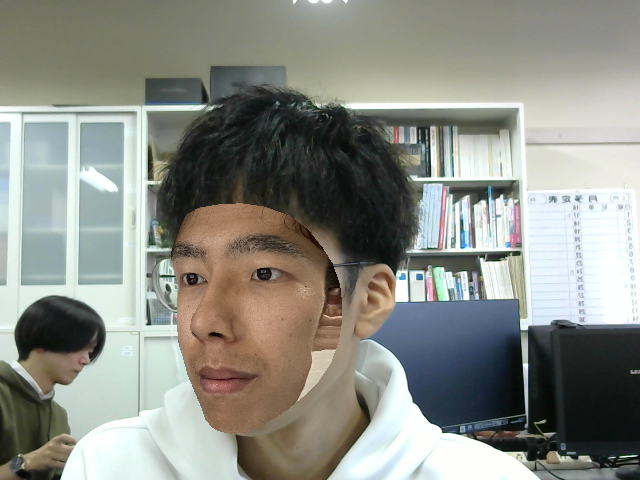
\includegraphics[keepaspectratio, scale=0.2]{figures/1.png}
      \caption{モデル変更前}
      \label{one}
    \end{minipage} &
    \begin{minipage}[t]{0.45\hsize}
      \centering
      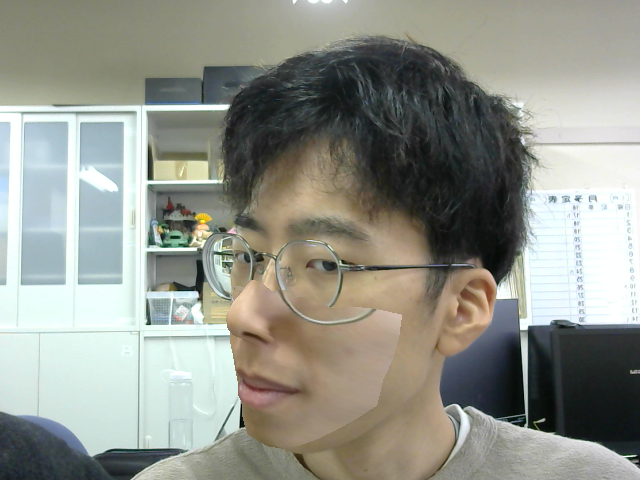
\includegraphics[keepaspectratio, scale=0.2]{figures/2.png}
      \caption{モデル変更後}
      \label{two}
    \end{minipage}
  \end{tabular}
\end{figure}
\\
また、ななめに撮影したときのテクスチャ画像を\hyperref[three]{図\ref{three}}とする。
このときの回転補正前の画像を\hyperref[four]{図\ref{four}}、補正後の画像を\hyperref[five]{図\ref{five}}とする。
少し分かりづらいが、回転の補正を行うことで正しく顔下部の切り抜きが行われていることがわかる。
ただ、$Y$軸、$Z$軸が反転してしまう問題や、テクスチャ画像をそのまま入力した場合正しくモデルが回転できないといった問題がある。
\begin{figure}[!ht]
  \begin{tabular}{ccc}
    \begin{minipage}[t]{0.3\hsize}
      \centering
      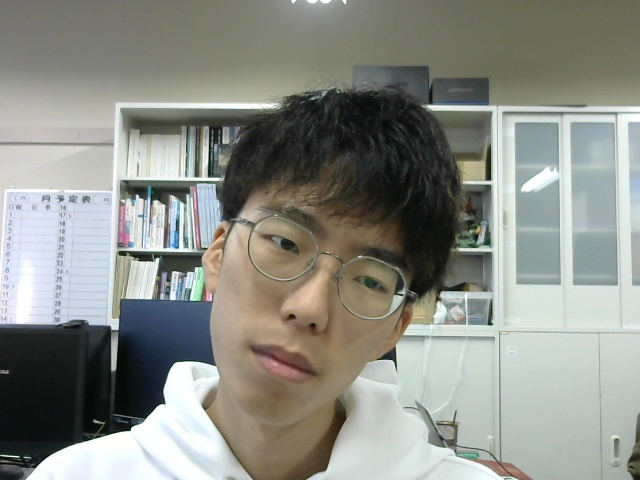
\includegraphics[keepaspectratio, scale=0.2]{figures/texture.jpg}
      \caption{テクスチャ画像}
      \label{three}
    \end{minipage} &
    \begin{minipage}[t]{0.3\hsize}
      \centering
      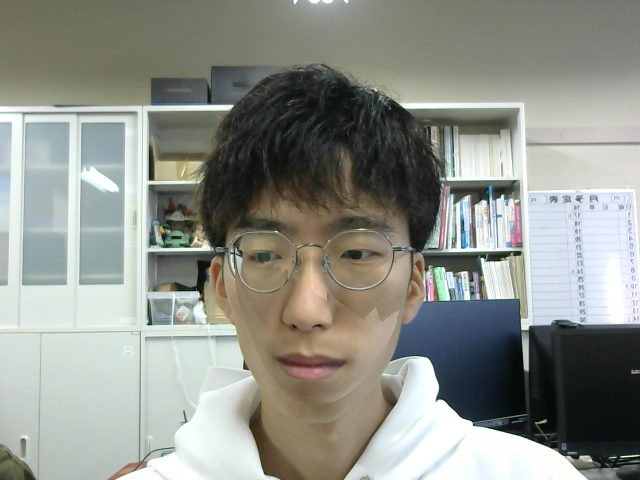
\includegraphics[keepaspectratio, scale=0.2]{figures/3.png}
      \caption{回転補正前}
      \label{four}
    \end{minipage}
    \begin{minipage}[t]{0.3\hsize}
      \centering
      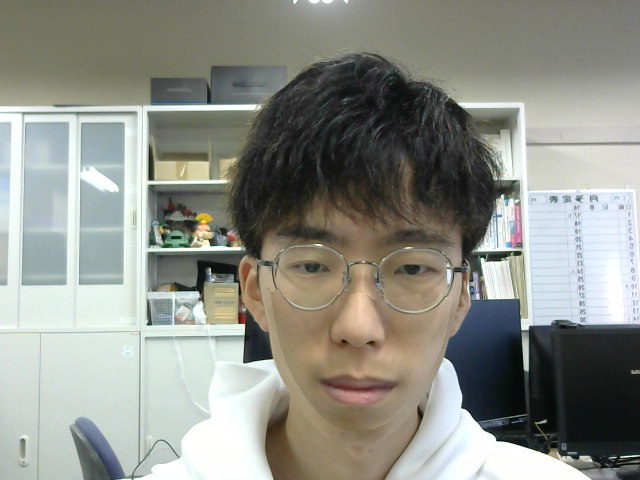
\includegraphics[keepaspectratio, scale=0.2]{figures/4.png}
      \caption{回転補正後}
      \label{five}
    \end{minipage}
  \end{tabular}
\end{figure}

\subsection{カメラ位置姿勢計算}
カメラ位置及び姿勢計算について、以下の三点で調整を行った。以降の節で詳細について説明する。
\begin{itemize}
  \item SolvePnPの初期値の設定
  \item 顔モデルの方向ベクトルを計算
  \item 顔モデルのオイラー角を計算
\end{itemize}

\subsection{SolvePnPの初期値の設定}
モデルが安定して表示されない問題を解決するために、SolvePnPの返り値である回転ベクトルと並進ベクトルがどのような値を出力しているか調べた。
結果として、並進ベクトルの$Z$の値の符号が繰り返し変化してしまっていることがわかった。これについて理由はわかっていないが、
問題を解決するアプローチとして、SolvePnPメソッドは初期値を指定することができるので、初期値として$Z=1000$とする。
これにより、$Z$の値の符号が固定され、処理が安定する。動画で処理の様子を比較する。\\

なお、カメラ位置姿勢計算に使う座標が4点の時は平面物体特徴量となり、初期値$Z$の値を決めない場合でも処理が安定する。
座標が6点以上の場合は空間物体特徴量となり、初期値$Z$の値を決める必要がある。
また、今回のプログラムではSolvePnPの計算方法として反復法を用いている。ほかの計算方法として遠近法や最小二乗法を使った
ものもあったが、安定しなかった。

\subsection{顔モデルの方向ベクトルを計算}
マスクをつけている際、顔の向きが安定しないという問題が発生していた。そのため、どのような向きになっているかを確認するため、
顔の方向ベクトルを求める。
プログラムではOpenCVのprojectionPointsメソッドで鼻先の正面の三次元座標をカメラ視点に投影し、
鼻先の座標と引き算することで方向ベクトルを求める。
また方向ベクトルを基に、モデルの顔向きをOpenGLのウィンドウ上に表示する機能を追加した。
\hyperref[six]{図\ref{six}}に、モデルの顔向きを表示した様子を示す。
\begin{figure}[!ht]
  \begin{center}
    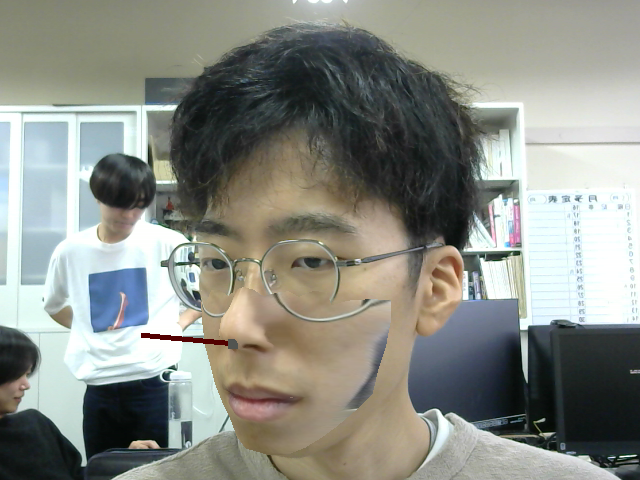
\includegraphics[scale=0.5]{figures/5.png}
    \caption{方向ベクトル}
    \label{six}
  \end{center}
\end{figure}
\\
\subsection{顔モデルのオイラー角を計算}
顔の向きが大きくなってしまうと顔検出の処理が安定しない問題が発生した。はじめは方向ベクトルでこの問題を解決しようと考えたが、
方向ベクトルの導出が安定せず、解決することができなかった。
そのため、顔モデルのオイラー角を計算し、その角度によってモデルを表示するかどうかを決定した。
プログラムではOpenCVのdecomposeProjectionMatrixメソッドで、オイラー角を求め、$XY$平面で光軸方向から左右25度以内の時
モデルを表示する。動画で処理の様子を表示する。\\
\newpage
\section{11月以降の目標}
11月以降の目標について以下にまとめる。\\
11月前半~12月
\begin{itemize}
  \item 論文執筆開始
  \item マスク着用を判定し、マスク着用時のランドマークの値を修正する。
\end{itemize}
%参考文献
\begin{thebibliography}{99}
\bibitem{bib_1} 菅谷保之,FaceMeshを利用した実寸サイズの3次元顔モデルの作成,閲覧日2023/7/26
\end{thebibliography}

\end{document}
